\documentclass[aspectratio=43,11pt]{beamer}

% ------------------------------------------------
% Pacchetti e setup
% ------------------------------------------------
\usetheme{Madrid}
\usecolortheme{default}
\usefonttheme{professionalfonts}

\usepackage[english]{babel}
\usepackage[T1]{fontenc}
\usepackage[utf8]{inputenc}
\usepackage{inconsolata} % font mono gradevole
\usepackage{listings}
\usepackage{xcolor}
\usepackage{graphicx}
\usepackage{algorithm}
\usepackage{algpseudocode}
\usepackage{float}
\usepackage{algorithm}%
\usepackage{algorithmicx}%
\usepackage{tikz}
\usepackage{multirow}
\usetikzlibrary{arrows.meta, shapes.geometric, positioning, fit, calc}

\algblock{ParallelFor}{EndParallelFor}
\algnewcommand\algorithmicparallelfor{\textbf{parallel for}}
\algnewcommand\algorithmicendparallelfor{\textbf{end parallel for}}
\algrenewtext{ParallelFor}[1]{\algorithmicparallelfor\ #1\ \algorithmicdo}
\algrenewtext{EndParallelFor}{\algorithmicendparallelfor}


% Meta
\title{Scaling Inter-procedural Dataflow Analysis on the Cloud}
\subtitle{Static Analysis and Software Verification}
\author{Simone Colli}
\date{2025-12-10}

% ------------------------------------------------
\begin{document}
% ------------------------------------------------

\begin{frame}
  \titlepage
\end{frame}

\begin{frame}{Index}
  \tableofcontents
\end{frame}

% ------------------------------------------------
\section{Introduction}
% ------------------------------------------------

\begin{frame}{Dataflow Analysis}{Introduction}
    \textbf{Definition}: Dataflow analysis is a static technique used to
    gather information about the possible set of values calculated at
    various points in a program.
    
    \vspace{0.5cm}
    
    Beyond compiler optimizations, dataflow analysis is widely used in:
    \begin{itemize}
      \item Bug detection.
      \item Security analysis.
    \end{itemize}

\end{frame}

\begin{frame}{Scalability}{Introduction}
    Applying inter-procedural dataflow analysis to large, real-world software
    presents major challenges:
    
    \vspace{0.5cm}
    
    \begin{enumerate}
        \item \textbf{Memory explosion}:
        Analysis tracks information at every program point.
        For precise analysis (e.g., context-sensitive alias analysis), the state size is huge.
      
        \item \textbf{Compute intensity}:
        Flow-sensitive analysis requires updating facts via transfer functions
        for every statement until convergence (Fixpoint).
    \end{enumerate}
    
\end{frame}

% \begin{frame}{BigDataflow}{Overview}
%     The paper introduces \textbf{BigDataflow}, a framework running on a cloud
%     cluster.
    
%     \vspace{0.5cm}
%     \textbf{Key Innovations:}
%     \begin{itemize}
%         \item \textbf{Distributed Vertex-Centric Model}: Adapting the worklist algorithm to run on graph processing engines (Apache Giraph).
%         \item \textbf{Optimization}: Pruning message passing to reduce network overhead.
%         \item \textbf{Incremental Analysis}: Handling code updates efficiently without re-analyzing the whole program.
%     \end{itemize}
    
%     \vspace{0.3cm}
%     \textbf{Result}: Analyzing Linux Kernel (17.5M LoC) in minutes instead of hours.
% \end{frame}

% ------------------------------------------------
\section{Background}
% ------------------------------------------------

\begin{frame}{Theoretical foundation}{Background}
    The framework relies on the standard Monotone Dataflow Analysis Framework.
    
    \begin{block}{Mathematical model}
    \begin{itemize}
        \item \textbf{Lattice} $L$: Represents the domain of abstract values.
        \item \textbf{Transfer function} $f$: $L \to L$. Models the effect of
        statements (e.g., $GEN/KILL$ sets).
        \item \textbf{Merge operator} $\sqcup$ (Join) or $\sqcap$ (Meet):
        Combines information from predecessors.
    \end{itemize}
    \end{block}
    
    The goal is to compute the \textbf{least fixpoint} (lfp) iteratively.
\end{frame}

\begin{frame}{Worklist algorithm}{Background}
    The standard sequential worklist algorithm iteratively updates
    dataflow facts:
    
    \begin{enumerate}
        \item Initialize all $IN$ sets to $\bot$.
        \item Add all CFG nodes to the worklist.
        \item While the worklist is not empty:
        \begin{itemize}
            \item Remove a node $k$ from the worklist.
            \item Compute $IN_k = \bigsqcup_{p \in preds(k)} OUT_p$.
            \item Compute $OUT_k = f_k(IN_k)$.
            \item If $OUT_k$ changed, add successors of $k$ to the worklist.
        \end{itemize}
    \end{enumerate}
    
    This continues until no more changes occur (fixpoint reached).

\end{frame}

\begin{frame}[fragile]{Worklist animation: Step 1}{Background}
    \begin{columns}[T]
        \begin{column}{0.5\textwidth}
            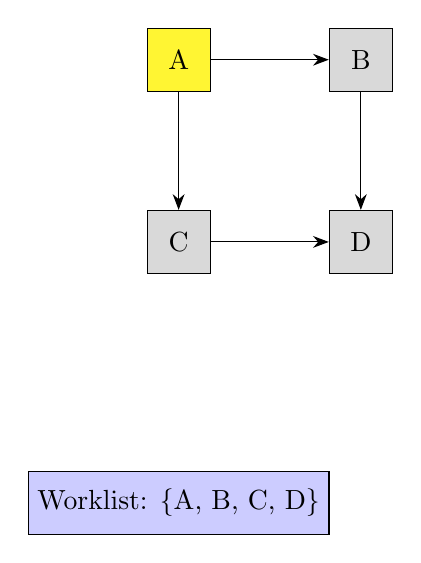
\begin{tikzpicture}[
                node distance=1.5cm,
                block/.style={rectangle, draw, minimum size=0.8cm},
                worklist/.style={rectangle, draw, fill=blue!20, minimum width=2cm, minimum height=0.8cm},
                active/.style={fill=yellow!80},
                inactive/.style={fill=gray!30}
            ]
                % CFG Nodes
                \node[block, active] (A) {A};
                \node[block, inactive, right=of A] (B) {B};
                \node[block, inactive, below=of A] (C) {C};
                \node[block, inactive, below=of B] (D) {D};

                % Edges
                \path[-{Stealth[length=2mm]}]
                    (A) edge (B)
                    (A) edge (C)
                    (B) edge (D)
                    (C) edge (D);
                
                % Worklist
                \node[worklist, below=of C, yshift=-1cm] (WL) {Worklist: \{A, B, C, D\}};
            \end{tikzpicture}
        \end{column}
        \begin{column}{0.5\textwidth}
            \begin{itemize}
                \item<1-> Initialize all $IN$ sets to $\bot$.
                \item<2-> Add all CFG nodes to the worklist.
            \end{itemize}
        \end{column}
    \end{columns}

    \begin{overprint}
        \onslide<1-2>
        \begin{figure}
        \centering
        \begin{tikzpicture}[overlay, remember picture]
            \node[opacity=0.1, text width=\textwidth] at (current page.center) {
                \begin{algorithmic}[1]
                    \scriptsize
                    \State Initialize all $IN$ sets to $\bot$.
                    \State Add all CFG nodes to the worklist.
                    \State While the worklist is not empty:
                    \begin{itemize}
                        \item Remove a node $k$ from the worklist.
                        \item Compute $IN_k = \bigsqcup_{p \in preds(k)} OUT_p$.
                        \item Compute $OUT_k = f_k(IN_k)$.
                        \item If $OUT_k$ changed, add successors of $k$ to the worklist.
                    \end{itemize}
                    \State This continues until no more changes occur (fixpoint reached).
                \end{algorithmic}
            };
        \end{tikzpicture}
        \end{figure}
    \end{overprint}
\end{frame}

\begin{frame}[fragile]{Worklist animation: Step 2}{Background}
    \begin{columns}[T]
        \begin{column}{0.5\textwidth}
            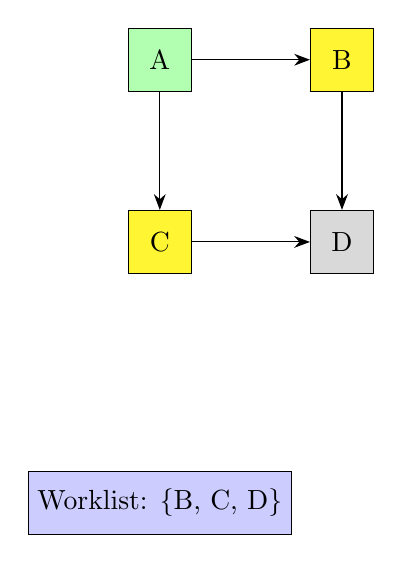
\begin{tikzpicture}[
                node distance=1.5cm,
                block/.style={rectangle, draw, minimum size=0.8cm},
                worklist/.style={rectangle, draw, fill=blue!20, minimum width=2cm, minimum height=0.8cm},
                active/.style={fill=yellow!80},
                inactive/.style={fill=gray!30},
                processed/.style={fill=green!30}
            ]
                % CFG Nodes
                \node[block, processed] (A) {A};
                \node[block, active, right=of A] (B) {B};
                \node[block, active, below=of A] (C) {C};
                \node[block, inactive, below=of B] (D) {D};

                % Edges
                \path[-{Stealth[length=2mm]}]
                    (A) edge (B)
                    (A) edge (C)
                    (B) edge (D)
                    (C) edge (D);
                
                % Worklist
                \node[worklist, below=of C, yshift=-1cm] (WL) {Worklist: \{B, C, D\}};
            \end{tikzpicture}
        \end{column}
        \begin{column}{0.5\textwidth}
            \begin{itemize}
                \item<1-> Remove A from worklist.
                \item<2-> Compute $IN_A$ (no predecessors).
                \item<3-> Compute $OUT_A = f_A(IN_A)$.
                \item<4-> $OUT_A$ changed, add B and C to worklist.
            \end{itemize}
        \end{column}
    \end{columns}

    \begin{overprint}
        \onslide<1-4>
        \begin{figure}
        \centering
        \begin{tikzpicture}[overlay, remember picture]
            \node[opacity=0.1, text width=\textwidth] at (current page.center) {
                \begin{algorithmic}[1]
                    \scriptsize
                    \State Initialize all $IN$ sets to $\bot$.
                    \State Add all CFG nodes to the worklist.
                    \State While the worklist is not empty:
                    \begin{itemize}
                        \item Remove a node $k$ from the worklist.
                        \item Compute $IN_k = \bigsqcup_{p \in preds(k)} OUT_p$.
                        \item Compute $OUT_k = f_k(IN_k)$.
                        \item If $OUT_k$ changed, add successors of $k$ to the worklist.
                    \end{itemize}
                    \State This continues until no more changes occur (fixpoint reached).
                \end{algorithmic}
            };
        \end{tikzpicture}
        \end{figure}
    \end{overprint}
\end{frame}

\begin{frame}[fragile]{Worklist animation: Step 3}{Background}
    \begin{columns}[T]
        \begin{column}{0.5\textwidth}
            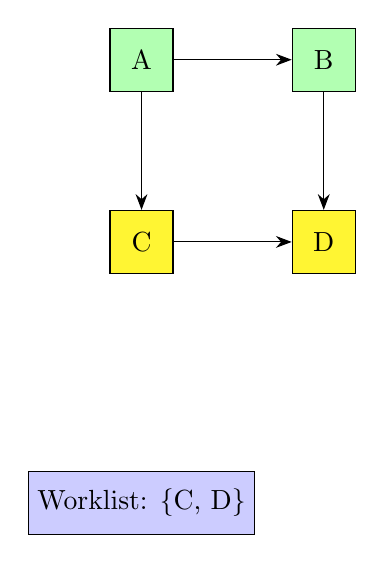
\begin{tikzpicture}[
                node distance=1.5cm,
                block/.style={rectangle, draw, minimum size=0.8cm},
                worklist/.style={rectangle, draw, fill=blue!20, minimum width=2cm, minimum height=0.8cm},
                active/.style={fill=yellow!80},
                inactive/.style={fill=gray!30},
                processed/.style={fill=green!30}
            ]
                % CFG Nodes
                \node[block, processed] (A) {A};
                \node[block, processed, right=of A] (B) {B};
                \node[block, active, below=of A] (C) {C};
                \node[block, active, below=of B] (D) {D};

                % Edges
                \path[-{Stealth[length=2mm]}]
                    (A) edge (B)
                    (A) edge (C)
                    (B) edge (D)
                    (C) edge (D);
                
                % Worklist
                \node[worklist, below=of C, yshift=-1cm] (WL) {Worklist: \{C, D\}};
            \end{tikzpicture}
        \end{column}
        \begin{column}{0.5\textwidth}
            \begin{itemize}
                \item<1-> Remove B from worklist.
                \item<2-> Compute $IN_B = OUT_A$.
                \item<3-> Compute $OUT_B = f_B(IN_B)$.
                \item<4-> $OUT_B$ changed, add D to worklist.
            \end{itemize}
        \end{column}
    \end{columns}

    \begin{overprint}
        \onslide<1-4>
        \begin{figure}
        \centering
        \begin{tikzpicture}[overlay, remember picture]
            \node[opacity=0.1, text width=\textwidth] at (current page.center) {
                \begin{algorithmic}[1]
                    \scriptsize
                    \State Initialize all $IN$ sets to $\bot$.
                    \State Add all CFG nodes to the worklist.
                    \State While the worklist is not empty:
                    \begin{itemize}
                        \item Remove a node $k$ from the worklist.
                        \item Compute $IN_k = \bigsqcup_{p \in preds(k)} OUT_p$.
                        \item Compute $OUT_k = f_k(IN_k)$.
                        \item If $OUT_k$ changed, add successors of $k$ to the worklist.
                    \end{itemize}
                    \State This continues until no more changes occur (fixpoint reached).
                \end{algorithmic}
            };
        \end{tikzpicture}
        \end{figure}
    \end{overprint}
\end{frame}

\begin{frame}[fragile]{Worklist animation: Step 4}{Background}
    \begin{columns}[T]
        \begin{column}{0.5\textwidth}
            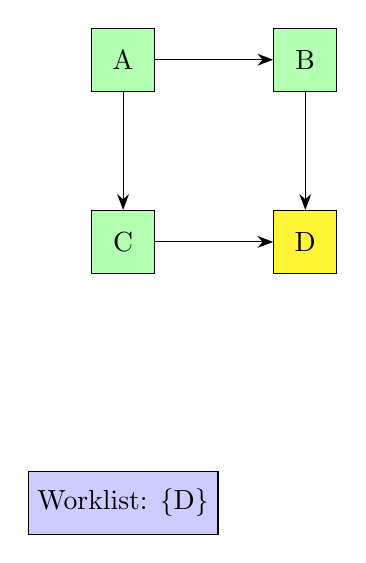
\begin{tikzpicture}[
                node distance=1.5cm,
                block/.style={rectangle, draw, minimum size=0.8cm},
                worklist/.style={rectangle, draw, fill=blue!20, minimum width=2cm, minimum height=0.8cm},
                active/.style={fill=yellow!80},
                inactive/.style={fill=gray!30},
                processed/.style={fill=green!30}
            ]
                % CFG Nodes
                \node[block, processed] (A) {A};
                \node[block, processed, right=of A] (B) {B};
                \node[block, processed, below=of A] (C) {C};
                \node[block, active, below=of B] (D) {D};

                % Edges
                \path[-{Stealth[length=2mm]}]
                    (A) edge (B)
                    (A) edge (C)
                    (B) edge (D)
                    (C) edge (D);
                
                % Worklist
                \node[worklist, below=of C, yshift=-1cm] (WL) {Worklist: \{D\}};
            \end{tikzpicture}
        \end{column}
        \begin{column}{0.5\textwidth}
            \begin{itemize}
                \item<1-> Remove C from worklist.
                \item<2-> Compute $IN_C = OUT_A$.
                \item<3-> Compute $OUT_C = f_C(IN_C)$.
                \item<4-> $OUT_C$ changed, add D to worklist (already there).
            \end{itemize}
        \end{column}
    \end{columns}

    \begin{overprint}
        \onslide<1-4>
        \begin{figure}
        \centering
        \begin{tikzpicture}[overlay, remember picture]
            \node[opacity=0.1, text width=\textwidth] at (current page.center) {
                \begin{algorithmic}[1]
                    \scriptsize
                    \State Initialize all $IN$ sets to $\bot$.
                    \State Add all CFG nodes to the worklist.
                    \State While the worklist is not empty:
                    \begin{itemize}
                        \item Remove a node $k$ from the worklist.
                        \item Compute $IN_k = \bigsqcup_{p \in preds(k)} OUT_p$.
                        \item Compute $OUT_k = f_k(IN_k)$.
                        \item If $OUT_k$ changed, add successors of $k$ to the worklist.
                    \end{itemize}
                    \State This continues until no more changes occur (fixpoint reached).
                \end{algorithmic}
            };
        \end{tikzpicture}
        \end{figure}
    \end{overprint}
\end{frame}

\begin{frame}[fragile]{Worklist animation: Step 5}{Background}
    \begin{columns}[T]
        \begin{column}{0.5\textwidth}
            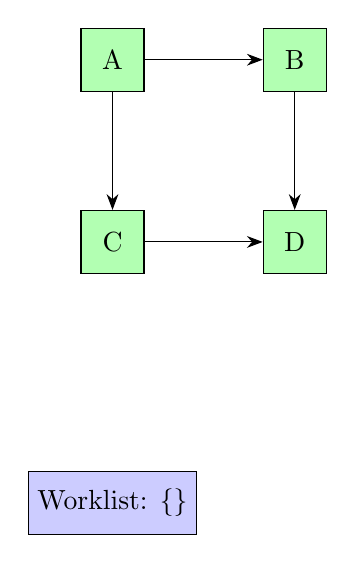
\begin{tikzpicture}[
                node distance=1.5cm,
                block/.style={rectangle, draw, minimum size=0.8cm},
                worklist/.style={rectangle, draw, fill=blue!20, minimum width=2cm, minimum height=0.8cm},
                active/.style={fill=yellow!80},
                inactive/.style={fill=gray!30},
                processed/.style={fill=green!30}
            ]
                % CFG Nodes
                \node[block, processed] (A) {A};
                \node[block, processed, right=of A] (B) {B};
                \node[block, processed, below=of A] (C) {C};
                \node[block, processed, below=of B] (D) {D};

                % Edges
                \path[-{Stealth[length=2mm]}]
                    (A) edge (B)
                    (A) edge (C)
                    (B) edge (D)
                    (C) edge (D);
                
                % Worklist
                \node[worklist, below=of C, yshift=-1cm] (WL) {Worklist: \{\}};
            \end{tikzpicture}
        \end{column}
        \begin{column}{0.5\textwidth}
            \begin{itemize}
                \item<1-> Remove D from worklist.
                \item<2-> Compute $IN_D = OUT_B \sqcup OUT_C$.
                \item<3-> Compute $OUT_D = f_D(IN_D)$.
                \item<4-> $OUT_D$ changed, add successors of D to worklist (none).
                \item<5-> Worklist is empty, fixpoint reached.
            \end{itemize}
        \end{column}
    \end{columns}

    \begin{overprint}
        \onslide<1-5>
        \begin{figure}
        \centering
        \begin{tikzpicture}[overlay, remember picture]
            \node[opacity=0.1, text width=\textwidth] at (current page.center) {
                \begin{algorithmic}[1]
                    \scriptsize
                    \State Initialize all $IN$ sets to $\bot$.
                    \State Add all CFG nodes to the worklist.
                    \State While the worklist is not empty:
                    \begin{itemize}
                        \item Remove a node $k$ from the worklist.
                        \item Compute $IN_k = \bigsqcup_{p \in preds(k)} OUT_p$.
                        \item Compute $OUT_k = f_k(IN_k)$.
                        \item If $OUT_k$ changed, add successors of $k$ to the worklist.
                    \end{itemize}
                    \State This continues until no more changes occur (fixpoint reached).
                \end{algorithmic}
            };
        \end{tikzpicture}
        \end{figure}
    \end{overprint}
\end{frame}

\begin{frame}{Vertex-centric graph processing}{Background}
    To distribute the analysis, the paper adopts the \textbf{vertex-centric
    model}.
    
    \vspace{0.3cm}
    The \textbf{GAS} model:
    \begin{itemize}
        \item \textbf{Gather}: A vertex collects data (messages) from
        neighbors (predecessors in CFG).
        \item \textbf{Apply}: The vertex updates its internal state
        (Dataflow fact) using the transfer function.
        \item \textbf{Scatter}: If the state changes, the vertex activates
        its neighbors (successors) and sends new messages.
    \end{itemize}
    
    \vspace{0.3cm}
    Mapping:
    \begin{itemize}
        \item Graph vertices $\to$ CFG basic blocks/statements.
        \item Vertex value $\to$ Abstract state ($IN$ and $OUT$ sets).
    \end{itemize}
\end{frame}


\begin{frame}[fragile]{Vertex-centric graph processing algorithm}{Background}
    \begin{algorithm}[H]
        \caption{The vertex-centric GAS model algorithm.}
        \label{alg:gas-algo}
        \begin{algorithmic}[1]
            \scriptsize
            \State \textbf{Data}: $\mathcal{A}$, the set of active vertices during processing
            \Repeat
                \ForAll{each vertex $k \in \mathcal{A}$ in parallel} \Comment{done by system}
                    \State Remove $k$ from $\mathcal{A}$ \Comment{done by system}
                    \State // Perform user-specified logic for each vertex
                    \State $\mathcal{M}_k \gets \text{Gather}(k)$ \Comment{gather messages or information from neighbors}
                    \State $\mathcal{D}_k \gets \text{Apply}(\mathcal{M}_k, k)$ \Comment{update value of k based on gathered information}
                    \State $\langle\mathcal{M}, \mathcal{A}'\rangle \gets \text{Scatter}(\mathcal{D}_k, k)$ \Comment{activate new vertices and/or send out messages}
                \EndFor
                \Statex \Comment{synchronize before next superstep}
                \State SYNCHRONIZE() \Comment{done by system}
                \State $\mathcal{A} \gets \mathcal{A}'$ \Comment{done by system}
            \Until{$\mathcal{A} = \emptyset$}
        \end{algorithmic}
    \end{algorithm}
\end{frame}

\begin{frame}[fragile]{GAS animation: superstep 1}{Background}
    \begin{columns}[T]
        \begin{column}{0.5\textwidth}
            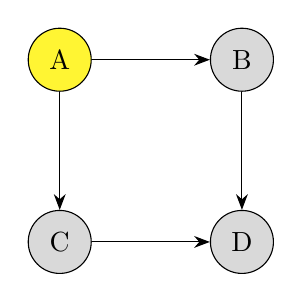
\begin{tikzpicture}[
                node distance=1.5cm,
                vertex/.style={circle, draw, minimum size=0.8cm},
                active/.style={fill=yellow!80},
                inactive/.style={fill=gray!30}
            ]
                % Nodes
                \node[vertex, active] (A) {A};
                \node[vertex, inactive, right=of A] (B) {B};
                \node[vertex, inactive, below=of A] (C) {C};
                \node[vertex, inactive, below=of B] (D) {D};

                % Edges
                \path[-{Stealth[length=2mm]}]
                    (A) edge (B)
                    (A) edge (C)
                    (B) edge (D)
                    (C) edge (D);
            \end{tikzpicture}
        \end{column}
        \begin{column}{0.5\textwidth}
            \begin{itemize}
                \item<1-> Initial state: Vertex A is active.
                \item<2-> A Gathers from neighbors (none).
                \item<3-> A Applies function, value changes.
                \item<4-> A Scatters to B and C, activating them.
            \end{itemize}
        \end{column}
    \end{columns}

    \begin{overprint}
        \onslide<1-4>
        \begin{figure}
        \centering
        \begin{tikzpicture}[overlay, remember picture]
            \node[opacity=0.1, text width=\textwidth] at (current page.center) {
                \begin{algorithmic}[1]
                    \scriptsize
                    % \State \textbf{Data}: $\mathcal{A}$, the set of active vertices during processing
                    \Repeat
                        \ForAll{each vertex $k \in \mathcal{A}$ in parallel} \Comment{done by system}
                            \State Remove $k$ from $\mathcal{A}$ \Comment{done by system}
                            \State // Perform user-specified logic for each vertex
                            \State $\mathcal{M}_k \gets \text{Gather}(k)$ \Comment{gather messages or information from neighbors}
                            \State $\mathcal{D}_k \gets \text{Apply}(\mathcal{M}_k, k)$ \Comment{update value of k based on gathered information}
                            \State $\langle\mathcal{M}, \mathcal{A}'\rangle \gets \text{Scatter}(\mathcal{D}_k, k)$ \Comment{activate new vertices and/or send out messages}
                        \EndFor
                        \Statex \Comment{synchronize before next superstep}
                        \State SYNCHRONIZE() \Comment{done by system}
                        \State $\mathcal{A} \gets \mathcal{A}'$ \Comment{done by system}
                    \Until{$\mathcal{A} = \emptyset$}
                \end{algorithmic}
            };
        \end{tikzpicture}
        \end{figure}
    \end{overprint}
\end{frame}

\begin{frame}[fragile]{GAS animation: superstep 2}{Background}
    \begin{columns}[T]
        \begin{column}{0.5\textwidth}
            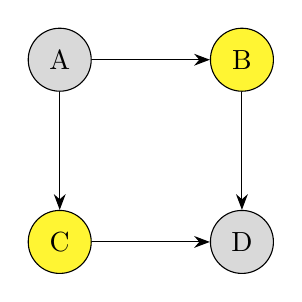
\begin{tikzpicture}[
                node distance=1.5cm,
                vertex/.style={circle, draw, minimum size=0.8cm},
                active/.style={fill=yellow!80},
                inactive/.style={fill=gray!30}
            ]
                % Nodes
                \node[vertex, inactive] (A) {A};
                \node[vertex, active, right=of A] (B) {B};
                \node[vertex, active, below=of A] (C) {C};
                \node[vertex, inactive, below=of B] (D) {D};

                % Edges
                \path[-{Stealth[length=2mm]}]
                    (A) edge (B)
                    (A) edge (C)
                    (B) edge (D)
                    (C) edge (D);
            \end{tikzpicture}
        \end{column}
        \begin{column}{0.5\textwidth}
            \begin{itemize}
                \item<1-> B and C are active.
                \item<2-> B and C Gather from A.
                \item<3-> B and C Apply function.
                \item<4-> B and C Scatter to D, activating it.
            \end{itemize}
        \end{column}
    \end{columns}

    \begin{overprint}
        \onslide<1-4>
        \begin{figure}
        \centering
        \begin{tikzpicture}[overlay, remember picture]
            \node[opacity=0.1, text width=\textwidth] at (current page.center) {
                \begin{algorithmic}[1]
                    \scriptsize
                    % \State \textbf{Data}: $\mathcal{A}$, the set of active vertices during processing
                    \Repeat
                        \ForAll{each vertex $k \in \mathcal{A}$ in parallel} \Comment{done by system}
                            \State Remove $k$ from $\mathcal{A}$ \Comment{done by system}
                            \State // Perform user-specified logic for each vertex
                            \State $\mathcal{M}_k \gets \text{Gather}(k)$ \Comment{gather messages or information from neighbors}
                            \State $\mathcal{D}_k \gets \text{Apply}(\mathcal{M}_k, k)$ \Comment{update value of k based on gathered information}
                            \State $\langle\mathcal{M}, \mathcal{A}'\rangle \gets \text{Scatter}(\mathcal{D}_k, k)$ \Comment{activate new vertices and/or send out messages}
                        \EndFor
                        \Statex \Comment{synchronize before next superstep}
                        \State SYNCHRONIZE() \Comment{done by system}
                        \State $\mathcal{A} \gets \mathcal{A}'$ \Comment{done by system}
                    \Until{$\mathcal{A} = \emptyset$}
                \end{algorithmic}
            };
        \end{tikzpicture}
        \end{figure}
    \end{overprint}
\end{frame}

\begin{frame}[fragile]{GAS animation: superstep 3}{Background}
    \begin{columns}[T]
        \begin{column}{0.5\textwidth}
            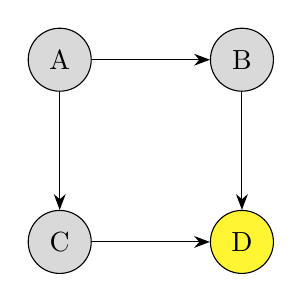
\begin{tikzpicture}[
                node distance=1.5cm,
                vertex/.style={circle, draw, minimum size=0.8cm},
                active/.style={fill=yellow!80},
                inactive/.style={fill=gray!30}
            ]
                % Nodes
                \node[vertex, inactive] (A) {A};
                \node[vertex, inactive, right=of A] (B) {B};
                \node[vertex, inactive, below=of A] (C) {C};
                \node[vertex, active, below=of B] (D) {D};

                % Edges
                \path[-{Stealth[length=2mm]}]
                    (A) edge (B)
                    (A) edge (C)
                    (B) edge (D)
                    (C) edge (D);
            \end{tikzpicture}
        \end{column}
        \begin{column}{0.5\textwidth}
            \begin{itemize}
                \item<1-> D is active.
                \item<2-> D Gather from B and C.
                \item<3-> D Apply function.
                \item<4-> D Scatter to nothing (no successors).
            \end{itemize}
        \end{column}
    \end{columns}

    \begin{overprint}
        \onslide<1-4>
        \begin{figure}
        \centering
        \begin{tikzpicture}[overlay, remember picture]
            \node[opacity=0.1, text width=\textwidth] at (current page.center) {
                \begin{algorithmic}[1]
                    \scriptsize
                    \State \textbf{Data}: $\mathcal{A}$, the set of active vertices during processing
                    \Repeat
                        \ForAll{each vertex $k \in \mathcal{A}$ in parallel} \Comment{done by system}
                            \State Remove $k$ from $\mathcal{A}$ \Comment{done by system}
                            \State // Perform user-specified logic for each vertex
                            \State $\mathcal{M}_k \gets \text{Gather}(k)$ \Comment{gather messages or information from neighbors}
                            \State $\mathcal{D}_k \gets \text{Apply}(\mathcal{M}_k, k)$ \Comment{update value of k based on gathered information}
                            \State $\langle\mathcal{M}, \mathcal{A}'\rangle \gets \text{Scatter}(\mathcal{D}_k, k)$ \Comment{activate new vertices and/or send out messages}
                        \EndFor
                        \Statex \Comment{synchronize before next superstep}
                        \State SYNCHRONIZE() \Comment{done by system}
                        \State $\mathcal{A} \gets \mathcal{A}'$ \Comment{done by system}
                    \Until{$\mathcal{A} = \emptyset$}
                \end{algorithmic}
            };
        \end{tikzpicture}
        \end{figure}
    \end{overprint}
\end{frame}

% -------------------------------------------------
\section{Methods}
% ------------------------------------------------


\begin{frame}{Proposed solutions}{Methods}

    Inspired by the GAS model, the paper designs the distributed vertex-centric
    worklist algorithm.
    \vspace{0.3cm}

    The paper proposes 2 frameworks:
    \begin{itemize}
        \item BigDataflow.
        \item BigDataflow-incremental.
    \end{itemize}
    Each in a classic and an optimized version:
    \begin{itemize}
        \item BigDataflow-classic.
        \item BigDataflow.
        \item BigDataflow-incremental.
        \item BigDataflow-incremental optimized.
    \end{itemize}
\end{frame}

\begin{frame}{System implementation}{Methods}
    BigDataflow is built on top of mature distributed systems to handle
    large-scale computation and state persistence.

%     \vspace{0.3cm}

    \begin{columns}[T]
        \begin{column}{0.48\textwidth}
            \begin{block}{Apache Giraph (Computation)}
                \begin{itemize}
                    \item \textbf{Role:} Executes the distributed worklist algorithms.
                    \item Functionality:
                    \begin{itemize}
                        \item \textbf{Partitions} the massive CFG across cluster nodes.
                        \item Manages \textbf{synchronization} (supersteps) and
                        message passing between workers.
                    \end{itemize}
                \end{itemize}
            \end{block}
        \end{column}

        \begin{column}{0.48\textwidth}
            \begin{block}{Redis (State storage)}
                \begin{itemize}
                    \item \textbf{Role:} Enabler for \textbf{incremental analysis}.
                    \item Functionality:
                    \begin{itemize}
                        \item Stores \textbf{whole-program analysis results}.
                        \item Allows low-latency \textbf{query} (for impact
                        analysis) and \textbf{update} of facts.
                    \end{itemize}
                \end{itemize}
            \end{block}
        \end{column}
    \end{columns}
\end{frame}

\begin{frame}[fragile]{BigDataflow-classic algorithm}{Methods}
    \begin{algorithm}[H]
        \caption{The BigDataflow-classic algorithm.}
        \label{alg:bigdataflow-classic}
        \begin{algorithmic}[1]
            \scriptsize
            \State \textbf{Data}: $\mathcal{W}$, the list of all active vertices during analysis; $DS_k: \{OUT_p | p \in preds(k)\}$ a set containing all the dataflow facts of k's predecessors
            \State $\mathcal{W} \gets \{\text{all the entry vertices in CFG}\}$
            \Repeat
                \ForAll{each CFG vertex $k \in \mathcal{W}$ do in parallel}
                    \State Remove $k$ from $\mathcal{W}$
                    \State $DS_k \gets \text{GATHERALL}(k)$ \Comment{gather all the predecessors' dataflow facts}
                    \State $IN'_k \gets \text{Merge}(DS_k)$ \Comment{merge}
                    \State $OUT'_k \gets \text{Transfer}(IN'_k, k)$ \Comment{transfer}
                    \If{Propagate($OUT_k, OUT'_k$)} \Comment{propagate}
                        \State $OUT_k \gets OUT'_k$
                        \State $\mathcal{W}' \gets \mathcal{W}' \cup \text{succs}(k)$
                    \EndIf
                \EndFor
                \State SYNCHRONIZE()
                \State $\mathcal{W} \gets \mathcal{W}'$
            \Until{$\mathcal{W} = \emptyset$}
        \end{algorithmic}
    \end{algorithm}
\end{frame}

\begin{frame}[fragile]{BigDataflow-classic animation}{Methods}
    \begin{tikzpicture}[
        remember picture,
        overlay,
        xshift=5cm, % Shift the entire graph to the right
        node distance=1.5cm,
        vertex/.style={circle, draw, minimum size=0.8cm},
        active/.style={fill=red!20},
        datastyle/.style={rectangle, draw}
    ]
        % Background algorithm
        \node[opacity=0.1, text width=\textwidth] at (current page.center) {
            \begin{algorithmic}[1]
                \scriptsize
                % \State \textbf{Data}: $\mathcal{W}$, the list of all active vertices during analysis; $DS_k: \{OUT_p | p \in preds(k)\}$ a set containing all the dataflow facts of k's predecessors
                \State $\mathcal{W} \gets \{\text{all the entry vertices in CFG}\}$
                \Repeat
                    \ForAll{each CFG vertex $k \in \mathcal{W}$ do in parallel}
                        \State Remove $k$ from $\mathcal{W}$
                        \State $DS_k \gets \text{GATHERALL}(k)$ \Comment{gather all the predecessors' dataflow facts}
                        \State $IN'_k \gets \text{Merge}(DS_k)$ \Comment{merge}
                        \State $OUT'_k \gets \text{Transfer}(IN'_k, k)$ \Comment{transfer}
                        \If{Propagate($OUT_k, OUT'_k$)} \Comment{propagate}
                            \State $OUT_k \gets OUT'_k$
                            \State $\mathcal{W}' \gets \mathcal{W}' \cup \text{succs}(k)$
                        \EndIf
                    \EndFor
                    \State SYNCHRONIZE()
                    \State $\mathcal{W} \gets \mathcal{W}'$
                \Until{$\mathcal{W} = \emptyset$}
            \end{algorithmic}
        };

        % Main graph nodes
        \node[vertex] (1) at (-2, 2) {1};
        \node[vertex] (2) at (0, 2) {2};
        \node[vertex] (3) at (2, 2) {3};
        \node[vertex, active] (4) at (0, 0) {4};
        \node[vertex] (5) at (-1, -2) {5};
        \node[vertex] (6) at (1, -2) {6};

        % Edges
        \path[-{Stealth[length=2mm]}]
            (1) edge (4)
            (2) edge (4)
            (3) edge (4)
            (4) edge (5)
            (4) edge (6);

        % Animation elements
        \visible<1>{
            \node[datastyle, right=of 4, yshift=0.7cm, xshift=0.1cm] (ds4) {$DS_4 = \{OUT'_1, OUT_2, OUT_3\}$};
            \coordinate (gather_start) at ($(ds4) + (0, 1cm)$);
            \draw[-{Stealth[length=2mm]}] (gather_start) -- (ds4) node[midway, right] {gather};
        }
        
        \visible<2>{
            \node[datastyle, right=of 4, yshift=0.7cm, xshift=0.1cm] (ds4) {$DS_4 = \{OUT'_1, OUT_2, OUT_3\}$};
            \node[datastyle, right=of 4, yshift=-0.5cm, xshift=2.25cm] (in4) {$IN'_4$};
            \coordinate (gather_start) at ($(ds4) + (0, 1cm)$);
            \draw[-{Stealth[length=2mm]}] (gather_start) -- (ds4) node[midway, right] {gather};
            \draw[-{Stealth[length=2mm]}] (ds4) -- (in4) node[midway, right] {merge};
        }
        
        \visible<3>{
            \node[datastyle, right=of 4, yshift=0.7cm, xshift=0.1cm] (ds4) {$DS_4 = \{OUT'_1, OUT_2, OUT_3\}$};
            \node[datastyle, right=of 4, yshift=-0.5cm, xshift=2.25cm] (in4) {$IN'_4$};
            \node[datastyle, right=of 4, yshift=-1.5cm, xshift=2.1cm] (out4_prime) {$OUT'_4$};
            \coordinate (gather_start) at ($(ds4) + (0, 1cm)$);
            \draw[-{Stealth[length=2mm]}] (gather_start) -- (ds4) node[midway, right] {gather};
            \draw[-{Stealth[length=2mm]}] (ds4) -- (in4) node[midway, right] {merge};
            \draw[-{Stealth[length=2mm]}] (in4) -- (out4_prime) node[midway, right] {transfer};
        }

        \visible<4>{
            \node[datastyle, right=of 4, yshift=0.7cm, xshift=0.1cm] (ds4) {$DS_4 = \{OUT'_1, OUT_2, OUT_3\}$};
            \node[datastyle, right=of 4, yshift=-0.5cm, xshift=2.25cm] (in4) {$IN'_4$};
            \node[datastyle, right=of 4, yshift=-1.5cm, xshift=2.1cm] (out4_prime) {$OUT'_4$};
            \coordinate (gather_start) at ($(ds4) + (0, 1cm)$);
            \draw[-{Stealth[length=2mm]}] (gather_start) -- (ds4) node[midway, right] {gather};
            \draw[-{Stealth[length=2mm]}] (ds4) -- (in4) node[midway, right] {merge};
            \draw[-{Stealth[length=2mm]}] (in4) -- (out4_prime) node[midway, right] {transfer};
            \node[vertex, active] (5) at (-1, -2) {5};
            \node[vertex, active] (6) at (1, -2) {6};
            \coordinate (arrow_end) at ($(out4_prime) + (0, -1.5cm)$);
            \draw[-{Stealth[length=2mm]}, thick, blue] (out4_prime) -- (arrow_end) node[midway, right] {\small propagate};

            % \draw[-{Stealth[length=2mm]}, thick] (out4_prime) -- (5) node[midway, above left] {propagate};
            % \draw[-{Stealth[length=2mm]}, thick] (out4_prime) -- (6) node[midway, above right] {propagate};
        }
    \end{tikzpicture}
\end{frame}
\begin{frame}{BigDataflow-classic limitations}{Methods}
\begin{tikzpicture}[
        remember picture,
        overlay,
        xshift=5cm, % Shift the entire graph to the right
        node distance=1.5cm,
        vertex/.style={circle, draw, minimum size=0.8cm},
        active/.style={fill=red!20},
        datastyle/.style={rectangle, draw}
    ]
        % Background algorithm
        \node[opacity=0.1, text width=\textwidth] at (current page.center) {
            \begin{algorithmic}[1]
                \scriptsize
                % \State \textbf{Data}: $\mathcal{W}$, the list of all active vertices during analysis; $DS_k: \{OUT_p | p \in preds(k)\}$ a set containing all the dataflow facts of k's predecessors
                \State $\mathcal{W} \gets \{\text{all the entry vertices in CFG}\}$
                \Repeat
                    \ForAll{each CFG vertex $k \in \mathcal{W}$ do in parallel}
                        \State Remove $k$ from $\mathcal{W}$
                        \State $DS_k \gets \text{GATHERALL}(k)$ \Comment{gather all the predecessors' dataflow facts}
                        \State $IN'_k \gets \text{Merge}(DS_k)$ \Comment{merge}
                        \State $OUT'_k \gets \text{Transfer}(IN'_k, k)$ \Comment{transfer}
                        \If{Propagate($OUT_k, OUT'_k$)} \Comment{propagate}
                            \State $OUT_k \gets OUT'_k$
                            \State $\mathcal{W}' \gets \mathcal{W}' \cup \text{succs}(k)$
                        \EndIf
                    \EndFor
                    \State SYNCHRONIZE()
                    \State $\mathcal{W} \gets \mathcal{W}'$
                \Until{$\mathcal{W} = \emptyset$}
            \end{algorithmic}
        };


        \node[text width=0.8\textwidth, align=center, fill=white, fill opacity=0.9, text opacity=1, 
              rounded corners, inner sep=10pt] at (current page.center) {
            Despite that the algorithm succeeds in leveraging large-scale distributed computing
            resources to accelerate dataflow analysis, it suffers from poor scalability.
            \vspace{0.3cm}

            Each vertex gathers \textbf{all} predecessor facts in every superstep, leading to
            \textbf{redundant data transmission} and \textbf{high memory consumption}.
        };
    \end{tikzpicture}
\end{frame}

% \begin{frame}{BigDataflow}{Methods}
%     The paper proposes an optimized algorithm using \textbf{Delta Updates}.
    
%     \vspace{0.3cm}
%     \textbf{Key Idea (Accumulative Property):}
%     Instead of gathering all facts, gather only \textbf{the updated} facts from the previous superstep.
    
%     $$ IN'_k = IN_k \sqcup (\bigsqcup_{p \in P'(k)} OUT'_p) $$
    
%     \begin{itemize}
%         \item $P'(k)$: Set of predecessors that actually changed.
%         \item \textbf{Benefit}: Prunes redundant data transmission. Significant reduction in memory and network load.
%     \end{itemize}
%     This is proved to be sound for distributive problems (Theorem 1).
% \end{frame}

\begin{frame}{BigDataflow optimized}{Methods}
The optimized algorithm gathers only the \textbf{updated} dataflow facts from
predecessors in the previous superstep.
\vspace{0.3cm}

This approach is achieved via a push-based message passing mechanism
\end{frame}

\begin{frame}[fragile]{BigDataflow optimized algorithm}{Methods}
    \begin{algorithm}[H]
        \caption{The BigDataflow optimized algorithm.}
        \label{alg:bigdataflow-optimized}
        \begin{algorithmic}[1]
            \scriptsize
            % \State \textbf{Data}: $\mathcal{W}$, the list of all active vertices during analysis; $\mathcal{M}_k: \{OUT'_p | p \text{ is a predecessor of } k\}$ a set containing the dataflow facts of k's predecessors which are updated at previous superstep
            \State $\mathcal{W} \gets \{\text{all the entry vertices in CFG}\}$
            \Repeat
                \ForAll{each CFG vertex $k \in \mathcal{W}$ \textbf{do in parallel}}
                    \State Remove $k$ from $\mathcal{W}$
                    \State $\mathcal{M}_k \gets \text{GATHERMESSAGES}(k)$ \Comment{gather only updated dataflow facts}
                    \State $IN'_k \gets \text{Merge}(\mathcal{M}_k, IN_k)$ \Comment{merge}
                    \State $OUT'_k \gets \text{Transfer}(IN'_k, k)$ \Comment{transfer}
                    \If{Propagate($OUT_k, OUT'_k$)} \Comment{propagate}
                        \State $OUT_k \gets OUT'_k$
                        \ForAll{successor $d$ of $k$}
                            \State $\text{SENDMESSAGES}(d, OUT'_k)$ \Comment{send the updated dataflow facts}
                            \State $\mathcal{W}' \gets \mathcal{W}' \cup \{d\}$
                        \EndFor
                    \EndIf
                    \State $IN_k \gets IN'_k$
                \EndFor
                \State SYNCHRONIZE()
                \State $\mathcal{W} \gets \mathcal{W}'$
            \Until{$\mathcal{W} = \emptyset$}
        \end{algorithmic}
    \end{algorithm}
\end{frame}

\begin{frame}[fragile]{BigDataflow optimized animation}{Methods}
    \begin{tikzpicture}[
        remember picture,
        overlay,
        xshift=5cm,
        node distance=1.5cm,
        vertex/.style={circle, draw, minimum size=0.8cm},
        active/.style={fill=red!20},
        datastyle/.style={rectangle, draw},
        msgstyle/.style={rectangle, draw, fill=blue!10}
    ]
        % Background algorithm
        \node[opacity=0.05, text width=0.9\textwidth, scale=0.7] at (current page.center) {
            \begin{algorithmic}[1]
                \scriptsize
                % \State \textbf{Data}: $\mathcal{W}$, the list of all active vertices during analysis; $\mathcal{M}_k: \{OUT'_p | p \text{ is a predecessor of } k\}$ a set containing the dataflow facts of k's predecessors which are updated at previous superstep
                \State $\mathcal{W} \gets \{\text{all the entry vertices in CFG}\}$
                \Repeat
                    \ForAll{each CFG vertex $k \in \mathcal{W}$ \textbf{do in parallel}}
                        \State Remove $k$ from $\mathcal{W}$
                        \State $\mathcal{M}_k \gets \text{GATHERMESSAGES}(k)$ \Comment{gather dataflow facts of the updated predecessors}
                        \State $IN'_k \gets \text{Merge}(\mathcal{M}_k, IN_k)$ \Comment{merge}
                        \State $OUT'_k \gets \text{Transfer}(IN'_k, k)$ \Comment{transfer}
                        \If{Propagate($OUT_k, OUT'_k$)} \Comment{propagate}
                            \State $OUT_k \gets OUT'_k$
                            \ForAll{successor $d$ of $k$}
                                \State $\text{SENDMESSAGES}(d, OUT'_k)$ \Comment{send the updated dataflow facts to successors}
                                \State $\mathcal{W}' \gets \mathcal{W}' \cup \{d\}$
                            \EndFor
                        \EndIf
                        \State $IN_k \gets IN'_k$
                    \EndFor
                    \State SYNCHRONIZE()
                    \State $\mathcal{W} \gets \mathcal{W}'$
                \Until{$\mathcal{W} = \emptyset$}
            \end{algorithmic}
        };

        % Main graph nodes
        \node[vertex] (1) at (-2, 2) {1};
        \node[vertex] (2) at (0, 2) {2};
        \node[vertex] (3) at (2, 2) {3};
        \node[vertex, active] (4) at (0, 0) {4};
        \node[vertex] (5) at (-1, -2) {5};
        \node[vertex] (6) at (1, -2) {6};

        % Edges
        \path[-{Stealth[length=2mm]}]
            (1) edge (4)
            (2) edge (4)
            (3) edge (4)
            (4) edge (5)
            (4) edge (6);

        % Animation elements
        \visible<1>{
            \node[msgstyle, right=of 4, yshift=0.7cm, xshift=0.1cm] (msg4) {$\mathcal{M}_4 = \{OUT'_1\}$};
            \coordinate (gather_start) at ($(msg4) + (0, 1cm)$);
            \draw[-{Stealth[length=2mm]}] (gather_start) -- (msg4) node[midway, right] {\small gather msgs};
            \node[above right=0.4cm of msg4, text=blue!70] {\scriptsize only updated!};
        }
        
        \visible<2>{
            \node[msgstyle, right=of 4, yshift=0.7cm, xshift=0.1cm] (msg4) {$\mathcal{M}_4 = \{OUT'_1\}$};
            \node[datastyle, right=of 4, yshift=-0.5cm, xshift=2.25cm] (in4) {$IN'_4$};
            \coordinate (gather_start) at ($(msg4) + (0, 1cm)$);
            \draw[-{Stealth[length=2mm]}] (gather_start) -- (msg4) node[midway, right] {\small gather msgs};
            \draw[-{Stealth[length=2mm]}] (msg4) -- (in4) node[midway, right] {merge};
        }
        
        \visible<3>{
            \node[msgstyle, right=of 4, yshift=0.7cm, xshift=0.1cm] (msg4) {$\mathcal{M}_4 = \{OUT'_1\}$};
            \node[datastyle, right=of 4, yshift=-0.5cm, xshift=2.25cm] (in4) {$IN'_4$};
            \node[datastyle, right=of 4, yshift=-1.8cm, xshift=2.1cm] (out4_prime) {$OUT'_4$};
            \coordinate (gather_start) at ($(msg4) + (0, 1cm)$);
            \draw[-{Stealth[length=2mm]}] (gather_start) -- (msg4) node[midway, right] {\small gather msgs};
            \draw[-{Stealth[length=2mm]}] (msg4) -- (in4) node[midway, right] {merge};
            \draw[-{Stealth[length=2mm]}] (in4) -- (out4_prime) node[midway, right] {transfer};
        }

        \visible<4>{
            \node[msgstyle, right=of 4, yshift=0.7cm, xshift=0.1cm] (msg4) {$\mathcal{M}_4 = \{OUT'_1\}$};
            \node[datastyle, right=of 4, yshift=-0.5cm, xshift=2.25cm] (in4) {$IN'_4$};
            \node[datastyle, right=of 4, yshift=-1.8cm, xshift=2.1cm] (out4_prime) {$OUT'_4$};
            \coordinate (gather_start) at ($(msg4) + (0, 1cm)$);
            \draw[-{Stealth[length=2mm]}] (gather_start) -- (msg4) node[midway, right] {\small gather msgs};
            \draw[-{Stealth[length=2mm]}] (msg4) -- (in4) node[midway, right] {merge};
            \draw[-{Stealth[length=2mm]}] (in4) -- (out4_prime) node[midway, right] {transfer};
            \node[vertex, active] (5) at (-1, -2) {5};
            \node[vertex, active] (6) at (1, -2) {6};
            \coordinate (arrow_end) at ($(out4_prime) + (0, -1.5cm)$);
            \draw[-{Stealth[length=2mm]}, thick, blue] (out4_prime) -- (arrow_end) node[midway, right] {\small send msg};
        }
    \end{tikzpicture}
\end{frame}



\begin{frame}{BigDataflow-incremental}{Methods}
    Real-world software changes frequently, especially in open-source projects.
    Re-analyzing from scratch is time-consuming and expensive.
    
    \vspace{0.3cm}
    \begin{figure}[H]
        \centering
        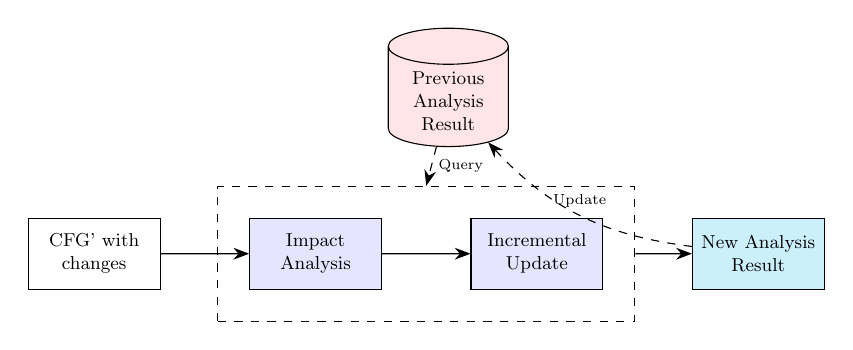
\begin{tikzpicture}[
            scale=0.75,
            transform shape,
            node distance=1.2cm and 1.5cm,
            block/.style={rectangle, draw, text width=2cm, align=center, minimum height=1.2cm, font=\small},
            db/.style={cylinder, shape border rotate=90, draw, text width=1.8cm, align=center, minimum height=0.8cm, aspect=0.3, fill=red!10, font=\small},
            proc/.style={rectangle, draw, fill=blue!10, text width=2cm, align=center, minimum height=1.2cm, font=\small}
        ]
            % Nodes
            \node[db] (prev) {Previous Analysis Result};
            \node[proc, below=of prev, xshift=1.5cm] (inc) {Incremental Update};
            \node[proc, left=of inc] (impact) {Impact Analysis};
            \node[block, left=of impact] (cfg) {CFG' with changes};
            \node[block, right=of inc, fill=cyan!20] (new) {New Analysis Result};

            % Dashed box
            \node[draw, dashed, fit=(impact) (inc), inner sep=0.4cm] (box) {};

            % Arrows
            \path[-{Stealth[length=2mm]}]
                (cfg) edge (impact)
                (impact) edge (inc)
                (box) edge (new);
            
            \path[-{Stealth[length=2mm]}, dashed]
                (prev) edge node[midway, right, text width=0.8cm, font=\scriptsize] {Query} (box.north)
                (new) edge[bend left=20] node[midway, above, font=\scriptsize] {Update} (prev);
                
        \end{tikzpicture}
        \caption{Workflow of Distributed Incremental Dataflow Analysis.}
        \label{fig:incremental-workflow}
    \end{figure}
    
\end{frame}

\begin{frame}{Workflow of BigDataflow-incremental}{Methods}
    
    \begin{figure}[H]
        \centering
        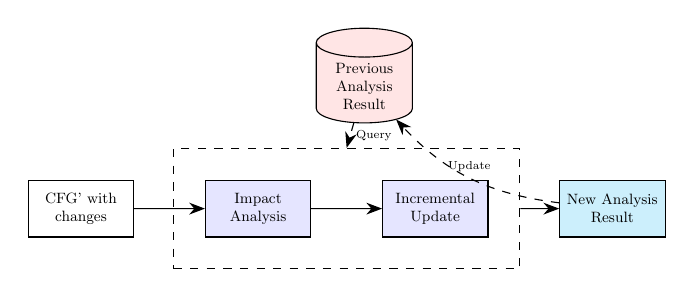
\begin{tikzpicture}[
            scale=0.60,
            transform shape,
            node distance=1.2cm and 1.5cm,
            block/.style={rectangle, draw, text width=2cm, align=center, minimum height=1.2cm, font=\small},
            db/.style={cylinder, shape border rotate=90, draw, text width=1.8cm, align=center, minimum height=0.8cm, aspect=0.3, fill=red!10, font=\small},
            proc/.style={rectangle, draw, fill=blue!10, text width=2cm, align=center, minimum height=1.2cm, font=\small}
        ]
            % Nodes
            \node[db] (prev) {Previous Analysis Result};
            \node[proc, below=of prev, xshift=1.5cm] (inc) {Incremental Update};
            \node[proc, left=of inc] (impact) {Impact Analysis};
            \node[block, left=of impact] (cfg) {CFG' with changes};
            \node[block, right=of inc, fill=cyan!20] (new) {New Analysis Result};

            % Dashed box
            \node[draw, dashed, fit=(impact) (inc), inner sep=0.4cm] (box) {};

            % Arrows
            \path[-{Stealth[length=2mm]}]
                (cfg) edge (impact)
                (impact) edge (inc)
                (box) edge (new);
            
            \path[-{Stealth[length=2mm]}, dashed]
                (prev) edge node[midway, right, text width=0.8cm, font=\scriptsize] {Query} (box.north)
                (new) edge[bend left=20] node[midway, above, font=\scriptsize] {Update} (prev);
                
        \end{tikzpicture}
        \caption{Workflow of Distributed Incremental Dataflow Analysis.}
        \label{fig:incremental-workflow-2}
    \end{figure}

    Given a \textbf{CFG with a batch of updates}, the framework:
    \begin{itemize}
        \item Performs \textbf{impact analysis} to identify affected nodes.
        \item Performs \textbf{incremental update}:
        \begin{itemize}
            \item Identification of affected nodes.
            \item Extraction of affected sub-CFGs.
            \item Re-analyzing only the affected sub-CFGs.
        \end{itemize}
        \item Produces the \textbf{new analysis result}.
    \end{itemize}

\end{frame}

% TODO descrivere brevemente il funzionamento di bigdataflow-incremental
\begin{frame}{BigDataflow-incremental}{Methods}
    The distributed incremental analysis reuses the existing analysis result
    and only performs local analysis on the updated parts to achieve
    efficiency.
    \vspace{0.1cm}
    \textbf{Atomic Changes:}
    The framework handles three categories of changes on the CFG:
    \begin{columns}[T]
        \begin{column}{0.48\textwidth}
            \begin{itemize}
                \item \textbf{Addition}:
                \begin{itemize}
                    \item Added edge between existing nodes.
                    \item Added source node and edge.
                    \item Added destination node.
                \end{itemize}
                \item \textbf{Deletion}:
                \begin{itemize}
                    \item Deleted edge.
                    \item Deleted source/destination node.
                \end{itemize}
            \end{itemize}
        \end{column}
        \begin{column}{0.48\textwidth}
            \begin{itemize}
                \item \textbf{Change}:
                \begin{itemize}
                    \item Changed source node (updates transfer function).
                    \item Changed destination node.
                \end{itemize}
            \end{itemize}
        \end{column}
    \end{columns}
    
    \vspace{0.1cm}
    These atomic changes trigger the \textbf{Impact Analysis} to identify
    the initial set of affected nodes.
\end{frame}

\begin{frame}[fragile]{BigDataflow-incremental algorithm steps}{Methods}
    \begin{algorithmic}[1]
        \scriptsize
        \State \textbf{Impact Analysis}: Identify directly affected nodes $\mathcal{A}$ based on atomic changes.
        \State \textbf{Transitive Closure}: $\mathcal{A} \leftarrow \mathcal{A} \cup \text{successors}(\mathcal{A})$.
        \State \textbf{Sub-CFG Construction}: Build $G'$ with nodes in $\mathcal{A}$ and connecting edges.
        \State \textbf{Initialization}: 
        \State \quad For $k \in \mathcal{A}_{add\_only}$: reuse previous results (Optimized).
        \State \quad For others: reset to $\bot$ or $\top$.
        \State \textbf{Boundary Handling}: Query $OUT$ facts from unaffected predecessors.
        \State \textbf{Incremental Update}: Run BigDataflow on $G'$.
    \end{algorithmic}
\end{frame}

\begin{frame}[fragile]{BigDataflow-incremental algorithm}{Methods}
    \begin{tikzpicture}[
        remember picture,
        overlay,
        xshift=5cm,
        node distance=1.5cm,
        vertex/.style={circle, draw, minimum size=0.8cm, fill=white},
        affected/.style={circle, draw, minimum size=0.8cm, fill=red!20},
        unaffected/.style={circle, draw, minimum size=0.8cm, fill=gray!10, draw=gray!40, text=gray!40},
        modified/.style={circle, draw, minimum size=0.8cm, fill=blue!30},
        newedge/.style={dashed, blue, thick},
        datastyle/.style={rectangle, draw, fill=white},
        msgstyle/.style={rectangle, draw, fill=blue!10}
    ]
        % Background algorithm text (always visible but faded)
        \node[opacity=0.1, text width=0.9\textwidth, scale=0.75] at (current page.center) {
            \begin{algorithmic}[1]
                \scriptsize
                \State \textbf{Impact Analysis}: Identify directly affected nodes $\mathcal{A}$
                \State \textbf{Transitive Closure}: $\mathcal{A} \leftarrow \mathcal{A} \cup \text{successors}(\mathcal{A})$
                \State \textbf{Sub-CFG Construction}: Build $G'$ with nodes in $\mathcal{A}$
                \State \textbf{Boundary Handling}: Query $OUT$ facts from unaffected predecessors
                \State \textbf{Incremental Update}: Run BigDataflow on $G'$
            \end{algorithmic}
        };

        % Base Graph Structure (nodes positions)
        \coordinate (pos1) at (-2, 2);
        \coordinate (pos2) at (0, 2);
        \coordinate (pos3) at (2, 2);
        \coordinate (pos4) at (0, 0);
        \coordinate (pos5) at (-1, -2);
        \coordinate (pos6) at (1, -2);

        % Step 1: Initial state with code change detected
        \only<1>{
            \node[vertex] (1) at (pos1) {1};
            \node[vertex] (2) at (pos2) {2};
            \node[vertex] (3) at (pos3) {3};
            \node[modified] (4) at (pos4) {4};
            \node[vertex] (5) at (pos5) {5};
            \node[vertex] (6) at (pos6) {6};
            
            \path[-{Stealth[length=2mm]}]
                (1) edge (4)
                (2) edge (4)
                (3) edge (4)
                (4) edge (5)
                (4) edge (6);
            
            \node[above=0.2cm of 4, text=blue, font=\small] {Modified!};
            \node[text width=4.5cm, align=left, font=\small] at (3.5, -1) {
                \textbf{Step 1}: Code change detected.\\
                Node 4 is modified
            };
        }

        % Step 2: Impact Analysis & Transitive Closure
        \only<2>{
            \node[vertex] (1) at (pos1) {1};
            \node[vertex] (2) at (pos2) {2};
            \node[vertex] (3) at (pos3) {3};
            \node[affected] (4) at (pos4) {4};
            \node[affected] (5) at (pos5) {5};
            \node[affected] (6) at (pos6) {6};
            
            \path[-{Stealth[length=2mm]}]
                (1) edge (4)
                (2) edge (4)
                (3) edge (4)
                (4) edge[red, thick] (5)
                (4) edge[red, thick] (6);
            
            \node[text width=4.5cm, align=left, font=\small] at (3.5, -1) {
                \textbf{Step 2}: Impact Analysis\\
                Identify affected node (4) and\\
                all transitive successors (5, 6)
            };
        }

        % Step 3: Sub-CFG Construction
        \only<3>{
            \node[unaffected] (1) at (pos1) {1};
            \node[unaffected] (2) at (pos2) {2};
            \node[unaffected] (3) at (pos3) {3};
            \node[affected] (4) at (pos4) {4};
            \node[affected] (5) at (pos5) {5};
            \node[affected] (6) at (pos6) {6};
            
            \path[-{Stealth[length=2mm]}, gray!40]
                (1) edge (4)
                (2) edge (4)
                (3) edge (4);
            \path[-{Stealth[length=2mm]}]
                (4) edge (5)
                (4) edge (6);
            
            \draw[red, dashed, very thick, rounded corners] (-1.8, 0.8) rectangle (1.8, -2.8);
            \node[red, font=\small, above] at (0, 0.8) {Sub-CFG $G'$};
            
            \node[text width=4.5cm, align=left, font=\small] at (4.5, -1) {
                \textbf{Step 3}: Sub-CFG Construction\\
                Extract affected nodes and edges\\
                Unaffected nodes are grayed out
            };
        }

        % Step 4: Boundary Handling & Re-analysis
        \only<4>{
            \node[unaffected] (1) at (pos1) {1};
            \node[unaffected] (2) at (pos2) {2};
            \node[unaffected] (3) at (pos3) {3};
            \node[affected] (4) at (pos4) {4};
            \node[affected] (5) at (pos5) {5};
            \node[affected] (6) at (pos6) {6};
            
            \path[-{Stealth[length=2mm]}, gray!40]
                (1) edge (4)
                (2) edge (4)
                (3) edge (4);
            \path[-{Stealth[length=2mm]}]
                (4) edge (5)
                (4) edge (6);
            
            % Boundary queries
            \node[msgstyle, above=0.3cm of 4, font=\scriptsize] (msg) {$OUT$ facts};
            \draw[-{Stealth[length=2mm]}, blue, thick] (msg) -- (4);
            
            \node[text width=4.5cm, align=left, font=\small] at (4, -0.5) {
                \textbf{Step 4}: Boundary \& Re-analysis\\
                Query $OUT$ facts from predecessors\\
                Run BigDataflow on Sub-CFG $G'$
            };
        }

    \end{tikzpicture}
\end{frame}
% ------------------------------------------------
\section{Results}
% ------------------------------------------------

\begin{frame}{Questions}{Results}
    The evaluation aims to answer the following questions:
    \begin{itemize}
        \item Q1: What is the overall performance of BigDataflow given a rich
        set of distributed computing resources?
        \item Q2: How does BigDataflow perform compared with other competitive analysis systems/tools?
        \item Q3: What about the performance of BigDataflow given the varying numbers of cores and
        resources?
        \item Q4: How about the performance of BigDataflow in the mode of incremental analysis?
    \end{itemize}
\end{frame}

\begin{frame}{Evaluation subjects}{Results}
    \begin{table}[H]
        \centering
        \caption{Subjects for evaluation}
        \label{tab:subjects}
        \small
        \begin{tabular}{|l|c|c|c|l|}
            \hline
            \textbf{Subject} & \textbf{Version} & \textbf{\#LoC} & \textbf{\#Functions} & \textbf{Description} \\
            \hline
            Linux & 5.2 & 17.5M & 565K & operating system \\
            Firefox & 67.0 & 7.9M & 770K & web browser \\
            PostgreSQL & 12.2 & 1.0M & 30K & database system \\
            OpenSSL & 1.1.1 & 519K & 12K & TLS protocol \\
            Httpd & 2.4.39 & 196K & 6K & web server \\
            \hline
        \end{tabular}
    \end{table}

    \vspace{0.3cm}
    Where \#LoC is the number of lines of code and \#Functions is the
    number of functions.
\end{frame}


\begin{frame}{Reference tools and hardware}{Results}
    \begin{table}[H]
        \centering
        \scriptsize
        \caption{Tools and hardware}
        \label{tab:tools-hardware}
        
        \begin{tabular}{|l|p{3cm}|p{4cm}|}
            \hline
            \textbf{Tool} & \textbf{Hardware} & \textbf{Description} \\
            \hline
            \textbf{BigDataflow-classic} (Baseline) & Cluster: 125 nodes (8
            vCPUs, 64GB RAM) & Classic distributed algorithm with full
            predecessor gathering \\
            \hline
            \textbf{BigDataflow} (Proposed) & Cluster: 125 nodes (8 vCPUs,
            64GB RAM) & Optimized with delta updates and message passing \\
            \hline
            \textbf{Chianina} (State-of-the-Art) & Single server (104 vCPUs,
            768GB RAM, 1TB SSD) & Parallel single-machine system with
            out-of-core support \\
            \hline
        \end{tabular}
    \end{table}
\end{frame}

\begin{frame}{Evaluation analysis}{Results}
    To test the performance and scalability of BigDataflow, two
    notoriously ``heavy'' dataflow analyses were chosen:

    \begin{block}{Context-sensitive alias analysis}
        Determines which pointers can point to the same memory location,
        considering the calling context of functions.
        It is computationally expensive because tracking every possible
        call path leads to an exponential explosion in the state space,
        resulting in massive memory consumption and long computation times.
    \end{block}

    \begin{block}{Instruction cache analysis}
        Predicts whether a machine instruction is likely to be in the CPU's
        instruction cache. It is memory-intensive as it requires modeling
        the cache behavior for all possible execution paths.
        The number of states can be enormous for large programs with
        complex control flow.
    \end{block}
\end{frame}

\begin{frame}[fragile]{Alias analysis}{Results}
    \tiny
    \begin{tabular}{|l|l|r|r|r|r|r|}
        \hline
        \textbf{Subject} & \textbf{Tool} & \textbf{\#PAliases} & \textbf{\#Workers/\#Part} & \textbf{\#PMem} & \textbf{Time} & \textbf{Cost (\$)} \\
        \hline
        \multirow{3}{*}{Linux} & BigDataflow & 12.5B & 350 & 3.5T & 16.7m & 11.1 \\
        & BigDataflow-classic & - & 350 & x & x & x \\
        & Chianina & - & 4 & 453.4G & 17.4h & 110.4 \\
        \hline
        \multirow{3}{*}{Firefox} & BigDataflow & 11.5B & 140 & 1.2T & 16.5m & 4.4 \\
        & BigDataflow-classic & - & 140 & x & x & x \\
        & Chianina & - & 4 & 131.6G & 5.3h & 33.6 \\
        \hline
        \multirow{3}{*}{PostgreSQL} & BigDataflow & 727.0M & 50 & 329.7G & 2.8m & 0.3 \\
        & BigDataflow-classic & - & 50 & 330.7G & 4.9m & 0.5 \\
        & Chianina & - & 1 & 61.9G & 50.4m & 5.3 \\
        \hline
        \multirow{3}{*}{OpenSSL} & BigDataflow & 734.8M & 30 & 285.3G & 3.5m & 0.2 \\
        & BigDataflow-classic & - & 30 & 329.8G & 6.8m & 0.4 \\
        & Chianina & - & 1 & 43.2G & 35.4m & 3.7 \\
        \hline
        \multirow{3}{*}{Httpd} & BigDataflow & 183.1M & 10 & 119.9G & 2.8m & 0.1 \\
        & BigDataflow-classic & - & 10 & 137.9G & 4.0m & 0.1 \\
        & Chianina & - & 1 & 14.2G & 11.2m & 1.2 \\
        \hline
    \end{tabular}

    \vspace{0.3cm}
    \normalsize
    Where \#PAliases is the number of pointer alias pairs discovered.
\end{frame}

\begin{frame}[fragile]{Instruction cache analysis}{Results}
    \tiny
    \begin{tabular}{|l|l|r|r|r|r|r|}
        \hline
        \textbf{Subject} & \textbf{Tool} & \textbf{\#BCached} & \textbf{\#Workers/\#Part} & \textbf{\#PMem} & \textbf{Time} & \textbf{Cost (\$)} \\
        \hline
        \multirow{3}{*}{Linux} & BigDataflow & 21.5B & 500 & 5.6T & 44.4m & 42.0 \\
        & BigDataflow-classic & - & 500 & x & x & x \\
        & Chianina & - & 4 & 555.4G & 9.4h & 59.6 \\
        \hline
        \multirow{3}{*}{Firefox} & BigDataflow & 15.8B & 400 & 4.4T & 39.0m & 29.5 \\
        & BigDataflow-classic & - & 400 & x & x & x \\
        & Chianina & - & 4 & 351.5G & 7.2h & 45.7 \\
        \hline
        \multirow{3}{*}{PostgreSQL} & BigDataflow & 1.4B & 180 & 1.1T & 3.2m & 1.1 \\
        & BigDataflow-classic & - & 180 & 1.1T & 6.5m & 2.2 \\
        & Chianina & - & 1 & 115.3G & 38.1m & 4.0 \\
        \hline
        \multirow{3}{*}{OpenSSL} & BigDataflow & 2.8B & 180 & 1.3T & 6.9m & 2.3 \\
        & BigDataflow-classic & - & 180 & 1.5T & 13.4m & 4.6 \\
        & Chianina & - & 1 & 227.6G & 1.7h & 10.8 \\
        \hline
        \multirow{3}{*}{Httpd} & BigDataflow & 782.0M & 100 & 684.3G & 3.0m & 0.6 \\
        & BigDataflow-classic & - & 100 & 781.3G & 4.6m & 0.9 \\
        & Chianina & - & 1 & 58.3G & 18.5m & 2.0 \\
        \hline
    \end{tabular}
    
    \vspace{0.3cm}
    \normalsize
    Where \#BCached is the number of blocks that may be cached.
\end{frame}

\begin{frame}{Scalability}{Results}
    \begin{figure}[H]
        \centering
        \includegraphics[width=0.8\textwidth]{scalab-alias.png}
        \caption{Scalability of BigDataflow on OpenSSL subject for alias
        analysis.}
        \label{fig:scalability-1}
    \end{figure}
    
\end{frame}
\begin{frame}{Scalability}{Results}
    \begin{figure}[H]
        \centering
        \includegraphics[width=0.8\textwidth]{scalab-cache.png}
        \caption{Scalability of BigDataflow on OpenSSL subject for cache
        analysis.}
        \label{fig:scalability-2}
    \end{figure}
    
\end{frame}

\begin{frame}[fragile]{Incremental analysis: Httpd-3days}{Results}
\begin{table}[h!]
\centering
\scriptsize
\setlength{\tabcolsep}{4pt}
\begin{tabular}{l | c c c c | c c c c}
\hline
\multirow{2}{*}{Subject} & \multicolumn{4}{c|}{BigDataflow-whole} & \multicolumn{4}{c}{BigDataflow-incremental} \\
\cline{2-9}
 & Cost & Time & \#Workers & \#PMem & Cost & Time & \#Workers & \#PMem \\
\hline
NU10 & \$0.643 & 3.4mins & 100 & 626.5G & \$0.038 & 1.0mins & 20 & 90.6G \\
NU9  & / & / & / & / & / & / & / & / \\
NU8  & \$0.662 & 3.5mins & 100 & 623.2G & \$0.129 & 1.7mins & 40 & 206.2G \\
NU7  & / & / & / & / & / & / & / & / \\
NU6  & \$0.681 & 3.6mins & 100 & 626.5G & \$0.030 & 0.8mins & 20 & 75.6G \\
NU5  & / & / & / & / & / & / & / & / \\
NU4  & / & / & / & / & / & / & / & / \\
NU3  & / & / & / & / & / & / & / & / \\
NU2  & / & / & / & / & / & / & / & / \\
NU1  & / & / & / & / & / & / & / & / \\
\hline
\end{tabular}
\end{table}

Where NU1 to NU10 are 10 consecutive updates to the Httpd
codebase over 3 days.

\end{frame}
% ------------------------------------------------
\section{Conclusion}
% ------------------------------------------------

\begin{frame}{Conclusion}
    BigDataflow addresses the scalability challenge of interprocedural
    dataflow analysis by leveraging cloud resources.
    
    \vspace{0.2cm}
    This work presents three key contributions:
    \begin{itemize}
        \item \textbf{Distributed Framework}: Adopts a vertex-centric graph
        model to distribute heavy computations across cluster nodes.
        \item \textbf{Algorithmic Innovation}:
        \begin{itemize}
            \item Optimized worklist: Prunes redundant data
            transmission via delta updates.
            \item Incremental analysis: Efficiently handles code
            updates, reducing cost and time by orders of magnitude.
        \end{itemize}
        \item \textbf{Usability}: Provides high-level APIs, allowing users
        to implement complex client analyses (e.g., Alias, Cache) easily.
    \end{itemize}
    
    \vspace{0.2cm}
    BigDataflow transforms ``intractable'' analysis tasks (e.g., analyzing
    17.5M LoC Linux Kernel) from hours to minutes, making deep
    software verification more viable for modern CI/CD pipelines.
\end{frame}

\begin{frame}
\centering
\vspace{2cm}
\huge
Thank you for your attention
\end{frame}

\end{document}